\chapter{Interactive and autonomous execution models}

\section{Engineering principles}

Interactive steering suits ambiguous tasks where human feedback changes the objective. Delegation suits well-specified, reversible work with observable completion conditions. Asynchronous execution is a scheduling property, not a security guarantee. Human-in-the-loop means a decision blocks progress until approval; human-on-the-loop means an operator can supervise without approving every step. Long-running work requires stable state and resumption rules.

\section{Implementation approach}

Score task ambiguity, reversibility, impact and verification strength on a low/medium/high scale. Use interactive exploration for unclear requirements, autonomous bounded runs for small changes with strong tests, and approval gates for high-impact operations. Split a risky migration into a read-only analysis, reviewed design, isolated rehearsal and separately authorized execution. Use the same task contract regardless of mode.

\section{Verification and limitations}

Escalate when the task exceeds scope or cannot produce objective evidence. Reassess the mode after new facts emerge; the original authorization does not automatically cover an expanded task.

Figure~\ref{fig:d10} illustrates the conceptual flow from Human task owner to Review evidence. The edges describe the proposed integration or control relationship, not undocumented internal calls.

\begin{figure}[htbp]\centering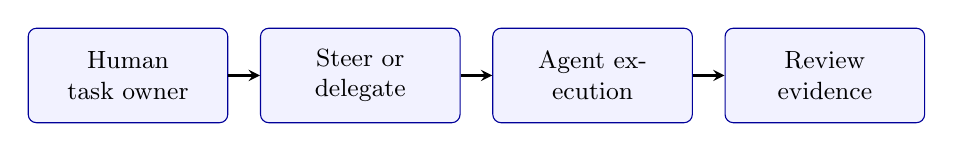
\begin{tikzpicture}[nodebox/.style={draw=blue!60!black,fill=blue!5,rounded corners=3pt,minimum height=12mm,text width=23mm,align=center,font=\small},>=stealth]
\node[nodebox] (n0) at (0.00,0.00) {Human task owner};
\node[nodebox] (n1) at (2.95,0.00) {Steer or delegate};
\node[nodebox] (n2) at (5.90,0.00) {Agent execution};
\node[nodebox] (n3) at (8.85,0.00) {Review evidence};
\draw[->,thick] (n0.east) -- (n1.west);
\draw[->,thick] (n1.east) -- (n2.west);
\draw[->,thick] (n2.east) -- (n3.west);
\end{tikzpicture}
\caption{Interactive and autonomous execution (conceptual view).}\label{fig:d10}\end{figure}

\section{Chapter conclusion}

Apply the stated verification criteria before expanding the scope of this workflow. Record deviations, evidence and unresolved risks in the task record.
